\subsection{Experiments setting}
For the experiments we used the Network Intrusion dataset~\cite{}, which consists of 494,021 instances.% described over 43 attributes. 
For the analysis, we used only the numerical attributes (\#34 out of \#43 attributes).

To evaluate the clustering quality, we report in Section~\ref{sec:expQuality}  on the sum of squares distance (SSQ) from the points to their nearest micro-cluster, using Euclidean distance as the distance function, within a horizon $H$.
We vary the speed of the stream and \color{red}the time window\color{black}.

With respect to the efficiency aspect, we report on \color{red}+++\color{black}, in Section~\ref{sec:expScalability}. 


% Two cases are analyzed in this section. These cases are two of the ones used by the developers of \textit{CluStream} to test its clustering capabilities. The tests differ in two ways: the speed of the stream and the time window used. The desired result would be to obtain comparable results for \textit{Spark-CluStream}.

\subsubsection{Results on clustering quality}
\label{sec:expQuality}
Depending on the speed of the stream and horizon, we derive two different stream configurations from our dataset.
The first one, denoted as $DS1$, has a speed $v=2,0000$ points per timestamp and a horizon $H=1$. This implies that the stream lasts for $\frac{494,021}{2,000} \approx 247$ time units.


% The measurement is the sum of squares (SSQ) of the euclidean distances from the points to their nearest macro-cluster. 
\color{red}In fact, the case is run a total of 4 times for \textit{Spark-CluStream} to compute an average. \color{black}
% The SSQ is defined as:
% \begin{equation}
%  SSQ = \sum_{i=1}^N distance(p_i,c)^2,
% \end{equation}
% where $N$ is the number of points used in the horizon $H=1$, which should average $N \approx 2000\cdot H \approx 2000$ points.

The parameters used in \cite{clustreamOrig} are: $\alpha=2,l=10,InitNumber=2000,\delta=512,t=2$.

\color{red}Omar, can you derive one figure with CluStream vs SparkClustream?\color{black}

\begin{figure}[h]
 \centering
 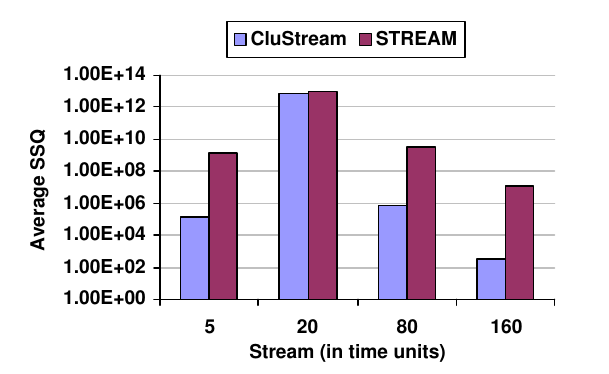
\includegraphics[scale=0.6]{./styles/2000h1-orig.png}
 % 2000h1-orig.png: 0x0 pixel, 300dpi, 0.00x0.00 cm, bb=
 \caption{Results for the original $CluStream$\cite{clustreamOrig}. Stream speed = 2000, H=1}
 \label{fig:2000orig}
\end{figure}

Figure \ref{fig:2000orig} shows the results used by the original \textit{CluStream} to show its capabilities against an older method \textit{STREAM}, which is a modified version of K-Means for data streams. The average SSQ for \textit{CluStream} is the most relevant to this test.

The parameters used for \textit{Spark-CluStream} were matched. 

\begin{figure}[h!]
 \centering
 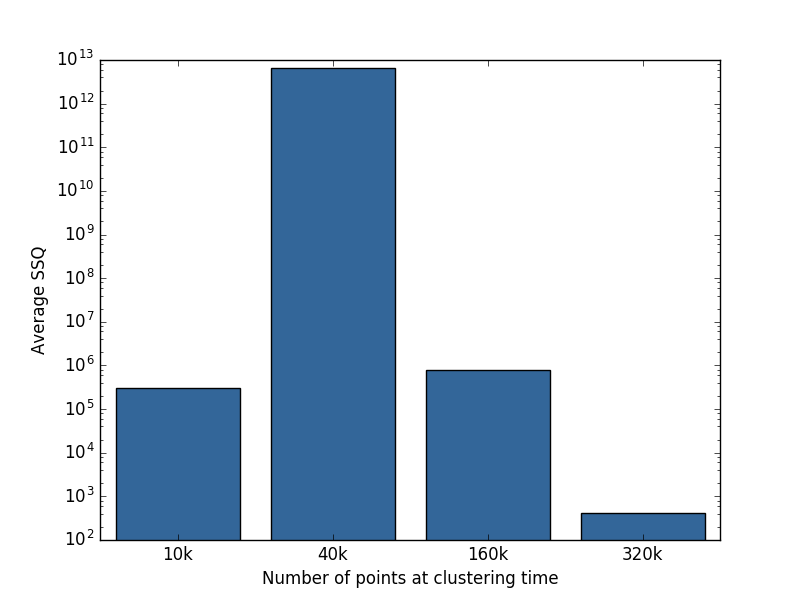
\includegraphics[scale=0.5]{./styles/2000h1.png}
 % 2000h1-orig.png: 0x0 pixel, 300dpi, 0.00x0.00 cm, bb=
 \caption{Validation results for $Spark-CluStream$. Stream speed = 2000, H=1}
 \label{fig:2000}
\end{figure}

The parameter $m$, for $m$ last points, was the only one not provided. Here, $m=20$ was chosen. For this case, both $m$ and $\delta$ are irrelevant and the reason is that the threshold is never reached (247 time units vs. 512). The number of micro-clusters $q$ is 50, a 10 times the number of final clusters (5) is enough for the vast majority of cases\cite{clustreamOrig}. The rest of the parameters were matched, with the only remaining thing to point out is that \textit{fakeKMeans()} used 5000 sampled points.

Figure \ref{fig:2000} shows the results obtained by \textit{Spark-CluStream}. There is a difference in the labels of the horizontal axis, while Figure \ref{fig:2000orig} shows the time units of the stream, Figure \ref{fig:2000orig} shows the number of points that had been streamed and processed. This is done because Spark streaming libraries in combination with the streaming simulation do not always deliver the same amount of points every single time unit, leading to inaccurate results comparing only by clustering on certain time units. A basic multiplication was used to determine the exact moment in terms of points: $2000\cdot 5 = 10000$, $2000\cdot 20 = 40000$ and so on.

Comparing the results, it is possible to deduce that they are very similar. The exact values for Figure \ref{fig:2000orig} are not available but it suffices to compare the magnitudes of the average SSQ. 

\begin{center}
\begin{tabular}{|l|l|l|l|l|}\hline
\textbf{Case 1: SSQ} & \textbf{10k} & \textbf{40k} & \textbf{160k} & \textbf{320k}\\\hline
CluStream & $10^5$-$10^6$ & $10^{12}$-$10^{13}$ & $\approx 10^6$ & $10^2$-$10^3$\\\hline
Spark-CluStream & $3.099\times10^5$ & $6.676\times10^{12}$ & $7.833\times10^5$ & $4.191\times10^2$\\\hline
\end{tabular}
\end{center}




\subsubsection{Results on DS2}

The second case uses a stream speed of 200 points per time unit and a horizon $H=256$. The dataset contains exactly 494021 points, meaning that the online phase would require $\frac{494021}{200} \approx 2470$ time units to complete.

The measurement is the SSQ again and the same circumstances apply for this case as in the first one with the difference that here $\delta$ and $m$ are relevant. The parameter $m$ is again chosen to be 20: if 200 points are processed every time unit and there are 50 micro-clusters, assuming all 200 points should be distributed uniformly at least every 5 time units leads to $5\frac{200}{50}=20$. An in-depth analysis of the behavior of \textit{CluStream} for different $\delta$'s and $m$'s is out of the scope of this work. 


\begin{figure}[h]
\hfill
\subfigure[\textit{Spark-CluStream}]{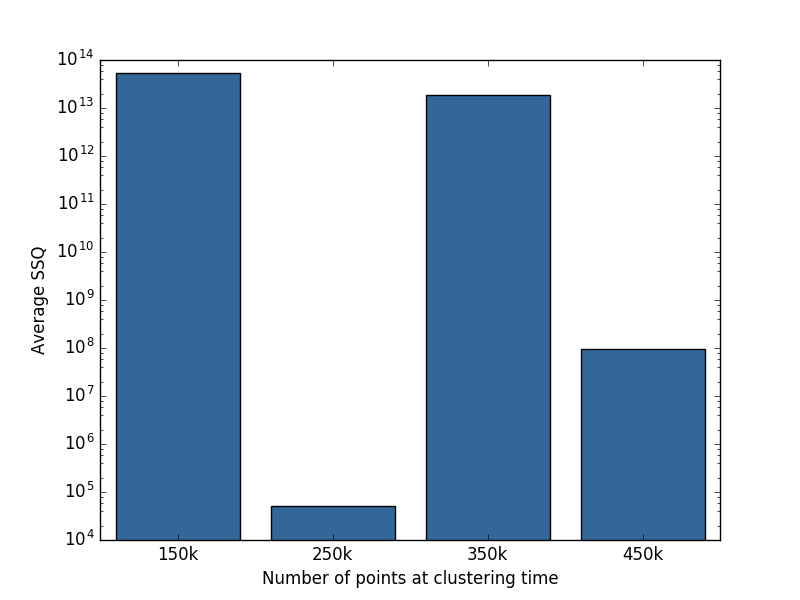
\includegraphics[width=5cm]{./styles/200h256.png}}
\hfill
\subfigure[Original \textit{CluStream}\cite{clustreamOrig}]{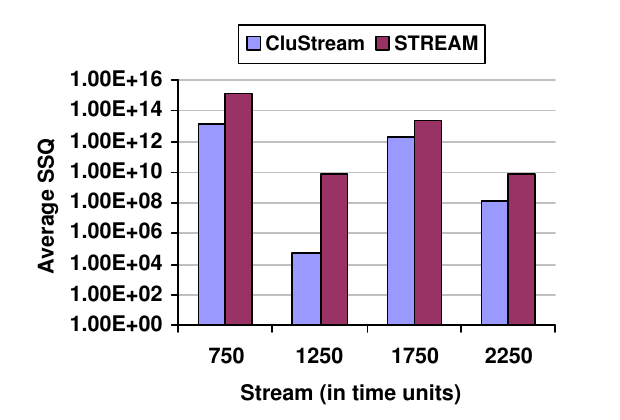
\includegraphics[width=5cm]{./styles/200h256-orig.png}}
\hfill
\caption{Validation results: case 2. Stream speed = 200, H = 256}
\label{fig:200h256}
\end{figure}

Again, the comparison is for the average SSQ. The test ran 4 times for \textit{Spark-CluStream} to average the results, which are very similar to the original \textit{CluStream} in this case as well:

\begin{center}
\begin{tabular}{|l|l|l|l|l|}\hline
\textbf{Case 2: SSQ} & \textbf{150k} & \textbf{250k} & \textbf{350k} & \textbf{450k}\\\hline
CluStream & $10^{13}$-$10^{14}$ & $\approx 10^{5}$ & $10^{12}$-$10^{13}$ & $\approx 10^{8}$\\\hline
Spark-CluStream & $5.402\times10^{13}$ & $5.143\times10^{4}$ & $1.892\times10^{13}$ & $9.646\times10^7$\\\hline
\end{tabular}
\end{center}



\subsubsection{Scalability}
\label{sec:expScalability}
The scalability tests are performed in two different scenarios: one being an analysis of how it scales for different number of attributes (dimensions of the data points) using only 20 micro-clusters and the other one using 200 micro-clusters. The reason behind this is that the number of attributes and the number of final clusters for a specific purpose are two key factors which determine the complexity of \textit{Spark-CluStream}. The speed of the stream is controlled for 10000 points for every batch of data because it is easier to test the scalability when many computations have to be done.

Any application using Spark streaming assigns one core exclusively to handle the stream, therefore the minimum number of processors required is two, this also means that using 2 processors is equivalent to using a single processor to execute the application. The number of processors mentioned in these tests is the total, but the real number of processors used for the computations is that number minus one.

\begin{figure}[h!]
 \centering
 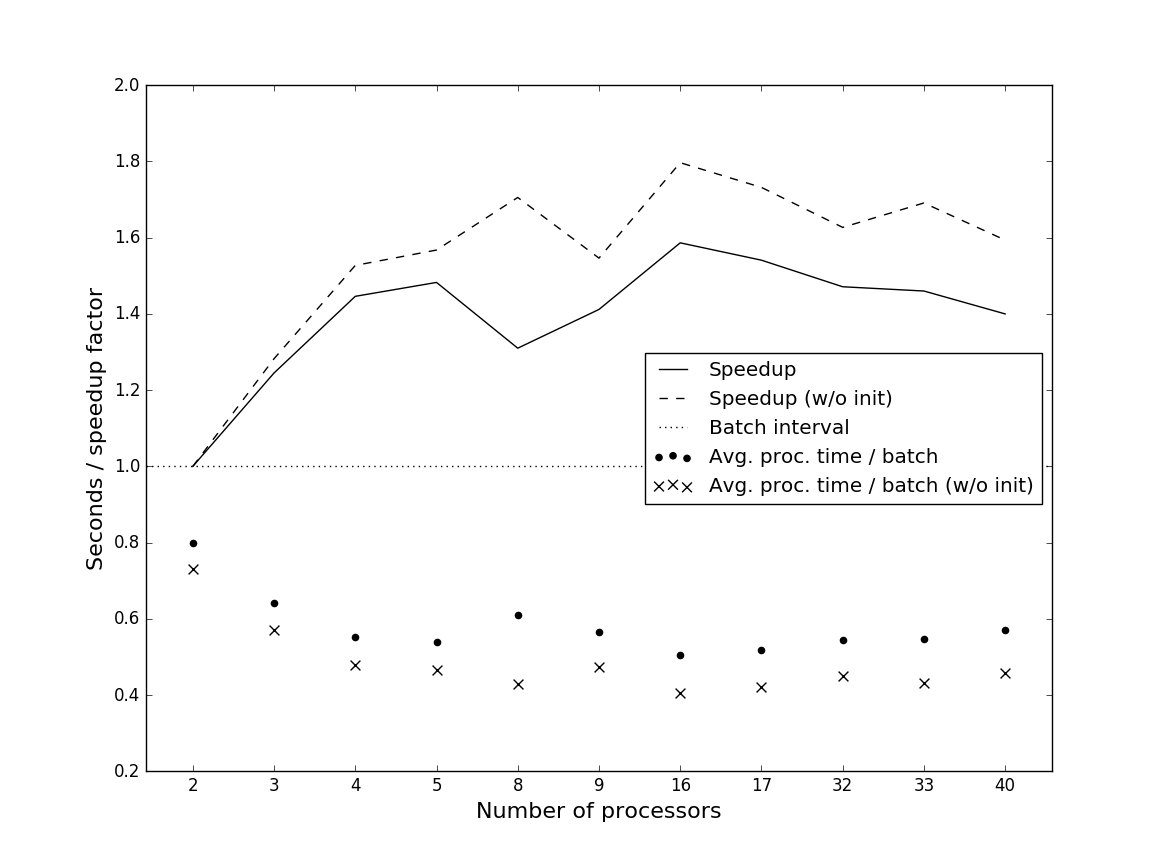
\includegraphics[scale=0.39]{./styles/perf20-2.png}
 \caption{Scalability: Stream speed = 10000, q = 20, d = 2}
 \label{fig:perf20-2}
\end{figure}


The charts here presented show the speedup obtained by increasing the number of processors from 2 to 40, which in reality means that 1 to 39 processors where used for the computations. It also shows the average processing time for each batch of data. Because the initialization takes the most amount of time, it is also convenient to show these values without considering that process: by doing so it is possible to see what would be the expected results for a longer run, where the initialization is no longer dominant. Finally it shows the interval time for which Spark process a new batch of data, in particular all these tests processed batch every second.



\begin{figure}[h!]
 \centering
 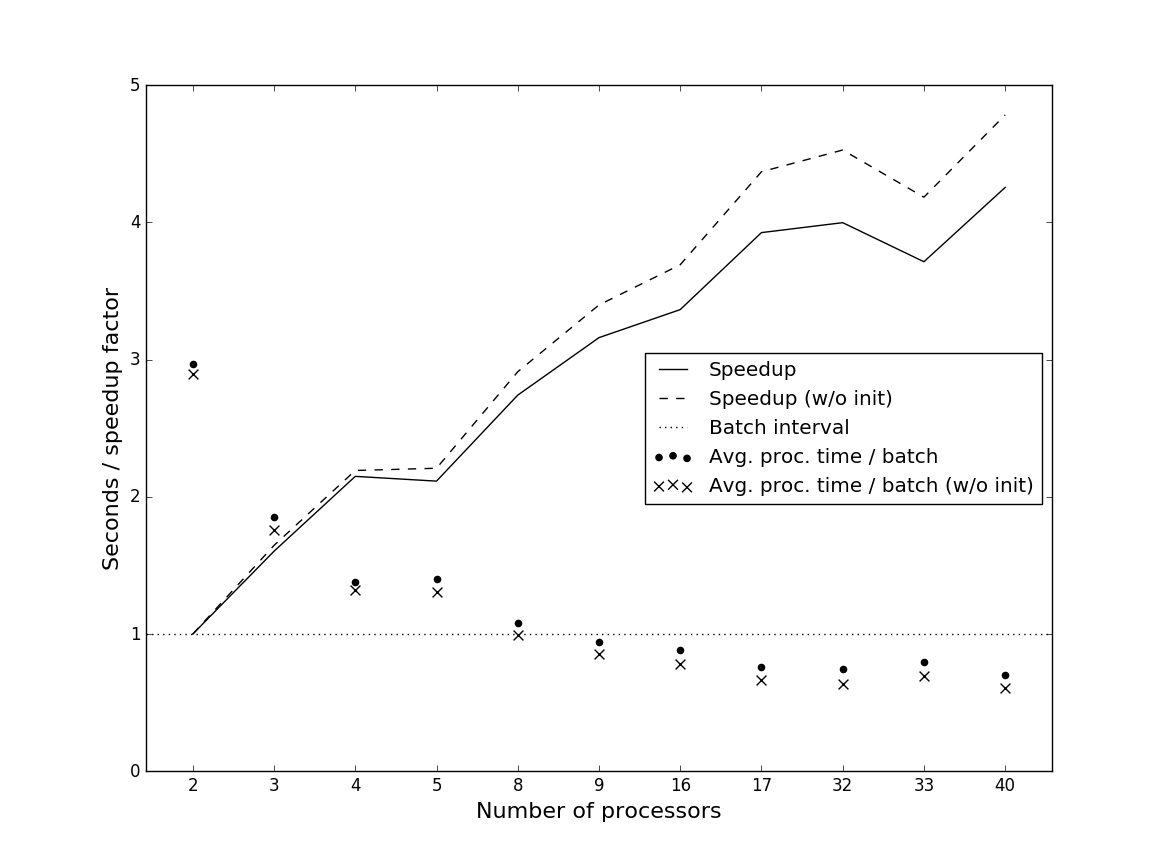
\includegraphics[scale=0.4]{./styles/perf20-100.png}
 \caption{Scalability: Stream speed = 10000, q = 20, d = 100}
 \label{fig:perf20-100}
\end{figure}


Figure \ref{fig:perf20-2} shows that using only 20 micro-clusters and 2 dimensions has poor scalability, not even being able to perform twice as fast as for a single processor (2 in total). Even for this high speed streaming, one processor is enough to process the batches of data before a new batch is processed, meaning that the setup is stable.

\begin{figure}[h!]
 \centering
 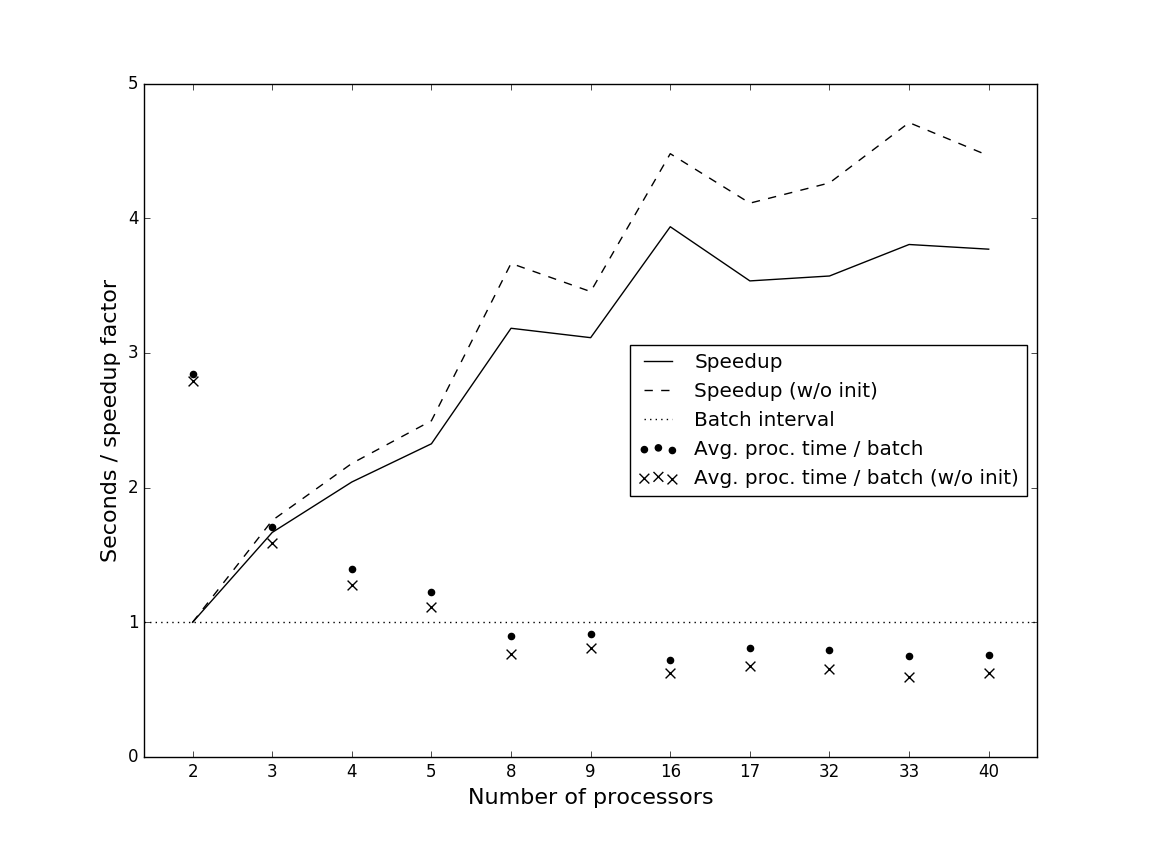
\includegraphics[scale=0.42]{./styles/perf200-2.png}
 \caption{Scalability: Stream speed = 10000, q = 200, d = 2}
 \label{fig:perf200-2}
\end{figure}

Increasing the dimensionality of the points increases the computational effort needed to process the points in every batch of data and here is where \textit{Spark-CluStream} shows its scalability, which is almost linear\footnote{By linear scalability does not mean it scales with a 1 to 1 ratio, but rather linearly proportional.} for up to 16-17 processors, as it can be seen in Figure \ref{fig:perf20-100}.  From the average processing time per batch, it can be seen that from 32 to 40 processors it does not improve much anymore and the speedup does not increase quasi-linearly anymore. Here a total of 9 processors were required to stabilize \textit{Spark-CluStream}. 

\begin{figure}[h!]
 \centering
 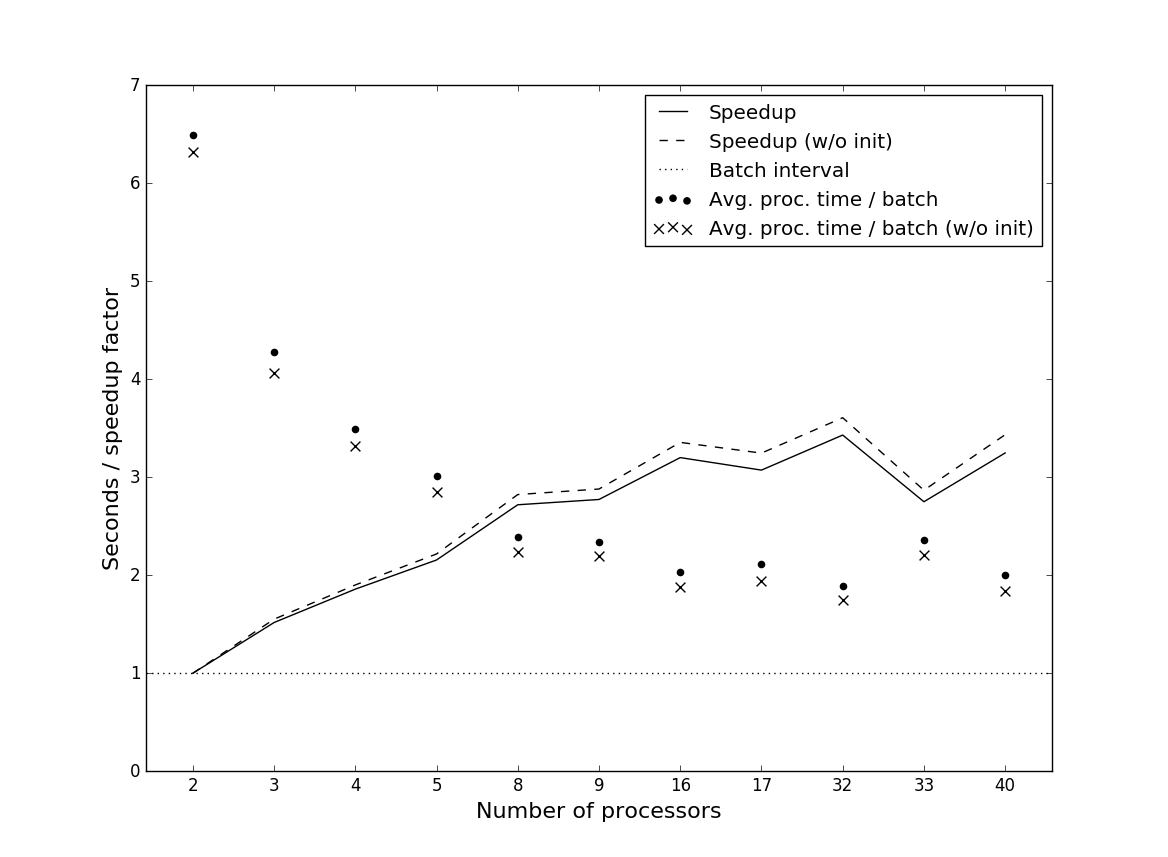
\includegraphics[scale=0.4]{./styles/perf200-100.png}
 \caption{Scalability: Stream speed = 10000, q = 200, d = 100}
 \label{fig:perf200-100}
\end{figure}

Interestingly, increasing the number of micro-clusters by a factor of 10 for 2 attributes resulted in good scalability, similarly to the scenario with 20 micro-clusters and 100 attributes. Here a total of 8 processors were enough for a stable run, as shown in Figure \ref{fig:perf200-2}.



Finally, when the number of clusters and the number of attributes are both increased significantly, Figure \ref{fig:perf200-100} shows for \textit{Spark-CluStream} quasi-linear scalability but this time only up to about 8-9 processors. After that point, the speedup slows down showing almost no improvement after 16 processors. This test never reached a stable configuration.

\subsubsection{Comparison against alternatives}

It is important for this project to know how \textit{Spark-CluStream} stands against some of the other alternatives for stream clustering available for Spark, in particular: \textit{Streaming K-Means} from Spark and \textit{StreamDM-CluStream}, which is another adaptation of the \textit{CluStream} method for Spark. There are two aspects of interest in this tests, one being their clustering capabilities and the other their performance.

\subsection{Clustering}

The setup and the dataset are the same as in \ref{validation}, as having already verified results provides the possibility of using those tests to directly compare the results against the other methods. Again, the used measurement is the sum of squares (SSQ).

Before looking at the results, here are some key considerations for the other methods:

\begin{itemize}
 \item \textit{Streaming K-Means}:
 \begin{itemize}
  \item In order to have comparable results, the time horizon $H$ must be interpreted differently. There are two strategies: the first option is to use the parameter \textit{halfLife}, which can be configured to let the algorithm to completely adjust the clusters after $HL$ points or batches.
  \item The alternative would be to set the $decayFactor$, which sets the weight for the clusters of the "old" data (only the current batch is considered "new" data). This is a number between 0 and 1, such that if it is 0 then only the clusters for "new" data determine the final clusters, if it is set to 1, then the clusters of past data will have the same influence on the final clusters. It is important to notice that this \textit{decayFactor} also considers the number of points of the "new" and "old" data, so in the last case, after a long time, "new" data will have little influence as the number of points of the current batch will be considerable smaller than the points clustered so far.
 \end{itemize}
 \item \textit{StreamDM-CluStream}:
 \begin{itemize}
  \item This adaptation of \textit{CluStream} does not include the offline part as a separate module, meaning that it does not save snapshots and therefore it has to perform the macro-clustering process for every batch. This brings some limitations, the horizon $H$ no longer has the same meaning: the $\delta$ parameter is used instead as an equivalent, relying on the micro-clustering part only and its ability to delete and create new micro-clusters.
\end{itemize}

\end{itemize}

\subsubsection{Case 1}

The parameters used for \textit{Spark-CluStream} are the same as in \ref{validation}. The number of clusters $k$ is always 5 for this dataset and these tests for all methods.

For \textit{Streaming K-Means}, the horizon $H=1$ was transformed to $halfLife=1000$ points. This is because the speed of the stream is 2000 points per time unit, if the horizon is 1, then only 2000 points are desired to be clustered, and half of that results in 1000 points. For the \textit{decayFactor}, it is safe to choose 0, as that would mean that only the last 2000 points have influence on the clusters, which is exactly what it's desired.

\textit{StreamDM-CluStream} is set up with its default parameters, only changing the horizon to 1 and the number of micro-clusters to 50 in order to match those of \textit{Spark-CluStream}.

\begin{figure}[h]
 \centering
 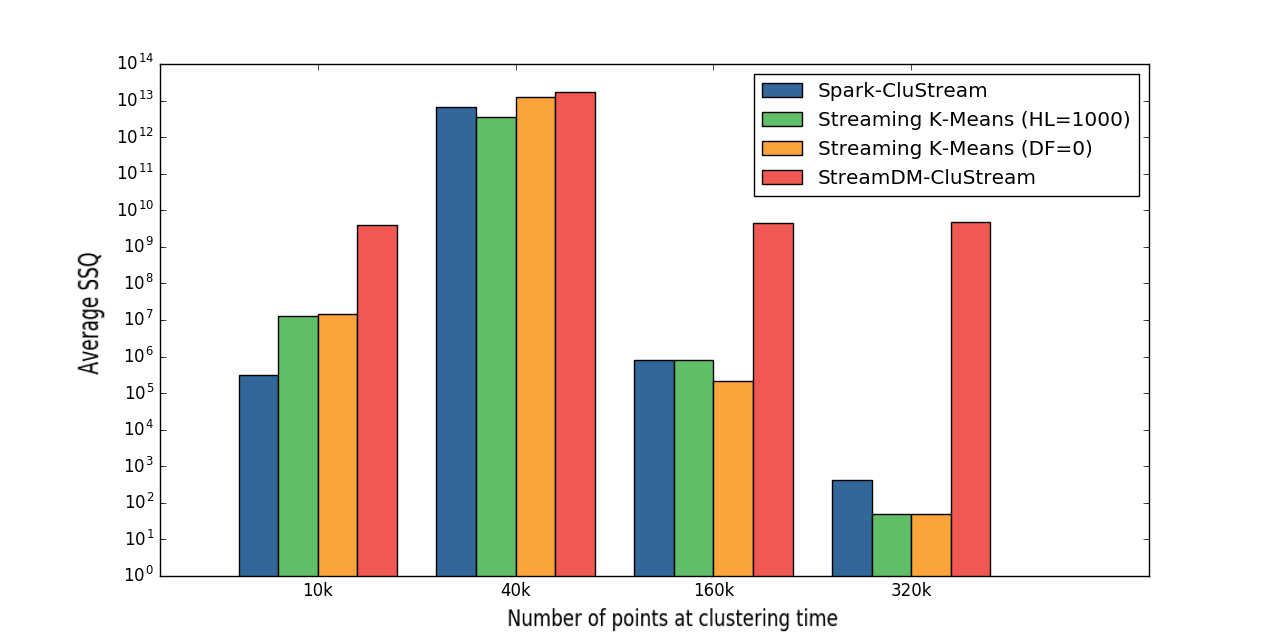
\includegraphics[scale=0.4]{./styles/comparison2000.png}
 \caption{Comparison results: all methods. Stream speed = 2000, H=1}
 \label{fig:comparison2000}
\end{figure}

From Figure \ref{fig:comparison2000} it can be seen that \textit{Spark-CluStream} delivers results which are very close to those of \textit{Streaming K-Means}, which performs significantly better than the older method \textit{STREAM}. Also, \textit{Streaming K-Means} with the \textit{decayFactor} (DF) is expected to do well on this test as it could be configured to cluster exactly as it was intended for this dataset. 

The surprising results came from \textit{StreamDM-CluStream}, as it performed noticeably, and significantly, worse than the rest of the methods. Specially for the last two marks at $160k$ and $320k$ it shows poor performance, which are where the other methods performed the better on average.

To find out whether this behavior is due to not using the snapshots plus offline macro-clustering, another test was performed using \textit{Spark-CluStream} with the same conditions as for \textit{StreamDM-CluStream}: using $\delta = 1$ as the horizon and $m=100$ to match both methods

\begin{figure}[h]
 \centering
 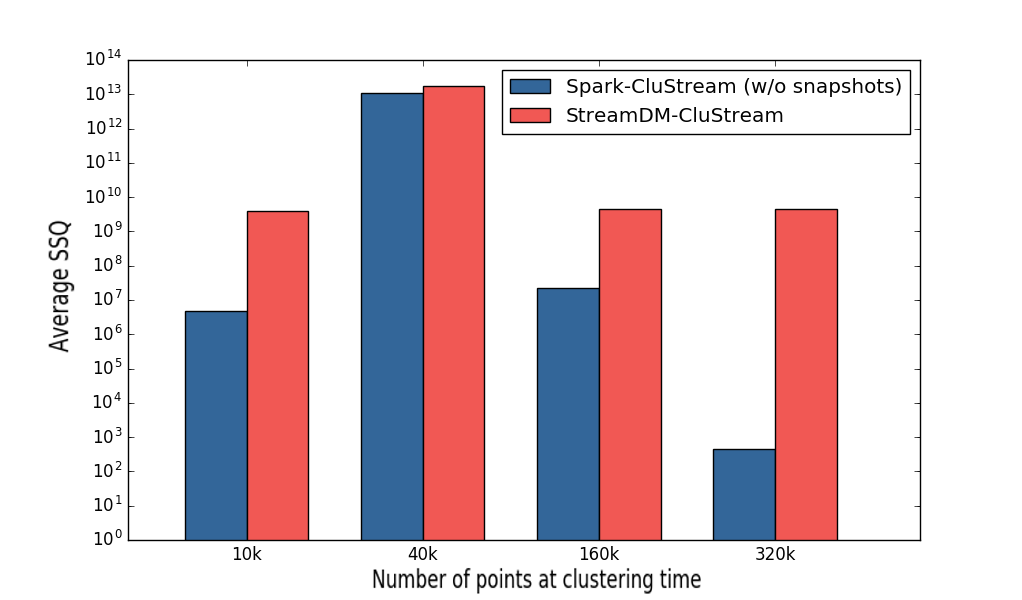
\includegraphics[scale=0.4]{./styles/comparisonNoSnaps.png}
 \caption{\textit{Spark-CluStream} without snapshots. Stream speed=2000, H=1, m=100}
 \label{fig:comparisonNoSnaps}
\end{figure}

Figure \ref{fig:comparisonNoSnaps} shows poorer results for \textit{Spark-CluStream} in comparison to its original behavior with snapshots, but still delivers noticeably better results than \textit{StreamDM-CluStream}, even though all these tests were executed 4 times and the SSQ erros were averaged to get a better representation of how these methods perform.

\subsubsection{Case 2}

Repeating the experiment for the stream with a speed of 200 and a horizon $H=256$ revealed unexpected results. While most parameters for all methods remained the same, for \textit{Streaming K-Means} a new $halfLife$ has to be calculated: multiplying the speed of the stream to the horizon, $200\cdot 256=51200$ shows how many points of the stream are supposed to be clustered at each time, indicating that the parameter should be set to $halfLife=25600$. 

\begin{figure}[h!]
 \centering
 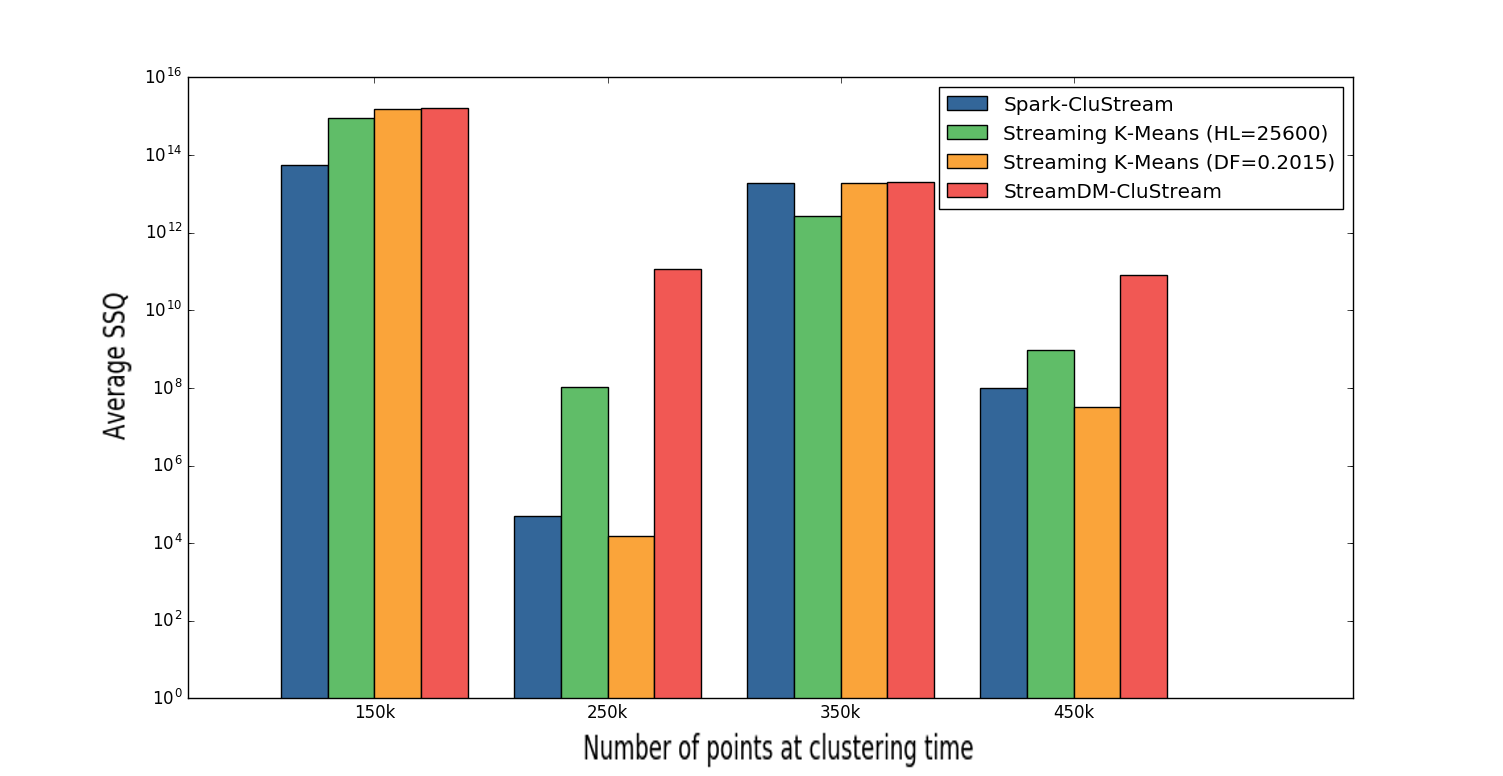
\includegraphics[scale=0.37]{./styles/comparison200.png}
 \caption{Comparison results: all methods. Stream speed = 200, H=256}
 \label{fig:comparison200}
\end{figure}

The \textit{decayFactor} strategy at first seems that does not work for such experiment, but considering that the total number of entries is known and exactly the marks at which the clustering process happens, it is possible to calculate an average value to use as a $decayFactor$: 

\begin{itemize}
 \item At 150000 points: $\frac{51200}{150000} \approx 0.3413$, which is the ratio of the points to cluster to the total number of points at that particular time.
 \item At 150000 points: $\frac{51200}{250000} \approx 0.2048$.
 \item At 150000 points: $\frac{51200}{350000} \approx 0.1462$.
 \item At 150000 points: $\frac{51200}{450000} \approx 0.1137$.
\end{itemize}

Averaging those ratios leads to a \textit{decayFactor = 0.2015}, which is a way to determine how important the old data is in comparison to the new one.


Figure \ref{fig:comparison200} shows that while \textit{Spark-CluStream} still performs consistently good, \textit{Streaming K-Means} with the \textit{decayFactor} outperformed its relative with the $halfLife$ strategy. Another thing to notice is that \textit{StreamDM-CluStream} still delivered the worse results. 

\begin{figure}[h]
 \centering
 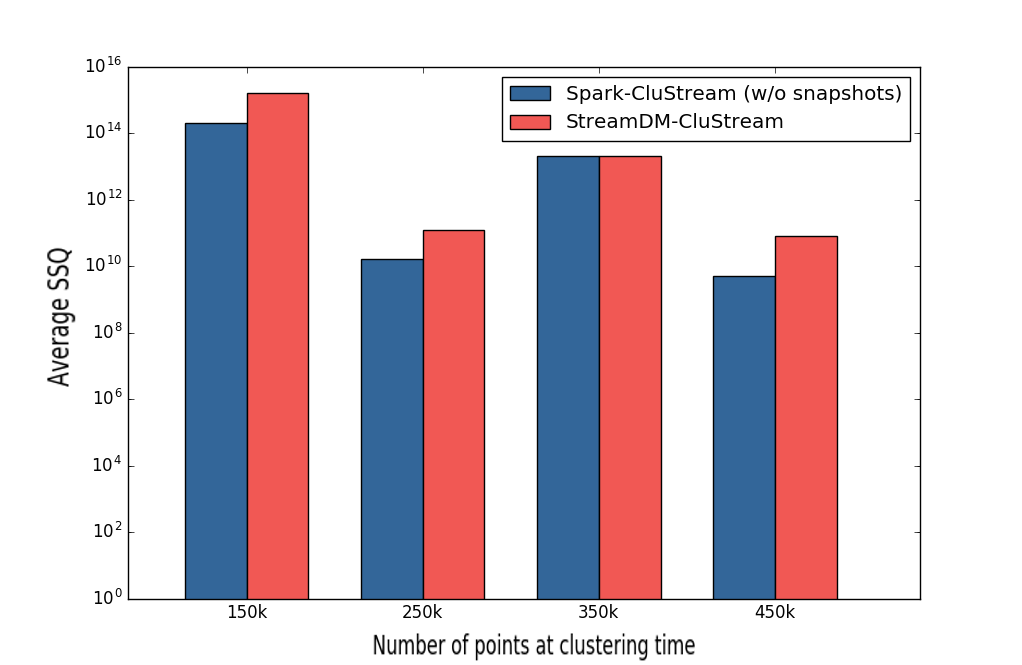
\includegraphics[scale=0.4]{./styles/comparisonNoSnaps2.png}
 \caption{\textit{Spark-CluStream} without snapshots. Stream speed = 200, H=256, m=100}
 \label{fig:comparisonNoSnaps2}
\end{figure}

Testing \textit{Spark-CluStream} again without the use of snapshots, showed once more that it delivers better results than \textit{StreamDM-CluStream}, as it can be seen in Figure \ref{fig:comparisonNoSnaps2}, but the difference was reduced significantly. These results might indicate that \textit{StreamDM-CluStream} does not benefit from shorter horizons.

\subsection{Performance}

In this section, the scalability of \textit{Spark-CluStream} is compared to that of \textit{StreamDM-CluStream} and Spark's \textit{Streaming K-Means} unsing the Spark cluster setup for $q=20$ and $d=2,100$, for the $CluStream$ method. Also, a test on a signle machine is performed, using the setup and dataset as in \ref{validation}.


\begin{figure}[h!]
 \centering
 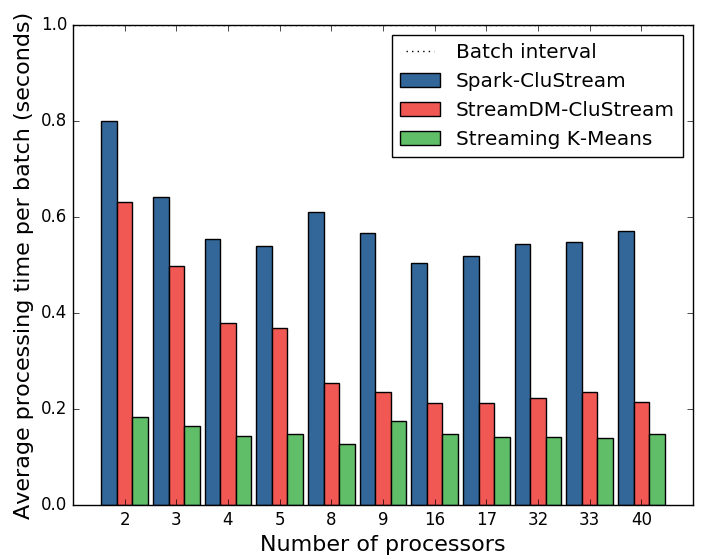
\includegraphics[scale=0.47]{./styles/perfComp2.png}
 \caption{Processing time comparison: $q=20$, $d=2$}
 \label{fig:perfComp2}
\end{figure}

In Figure \ref{fig:perfComp2} it can be seen that \textit{Spark-CluStream} took the most time on average to process a batch of data and being \textit{Streaming K-Means} the fastets among the three. 

\begin{figure}[h!]
 \centering
 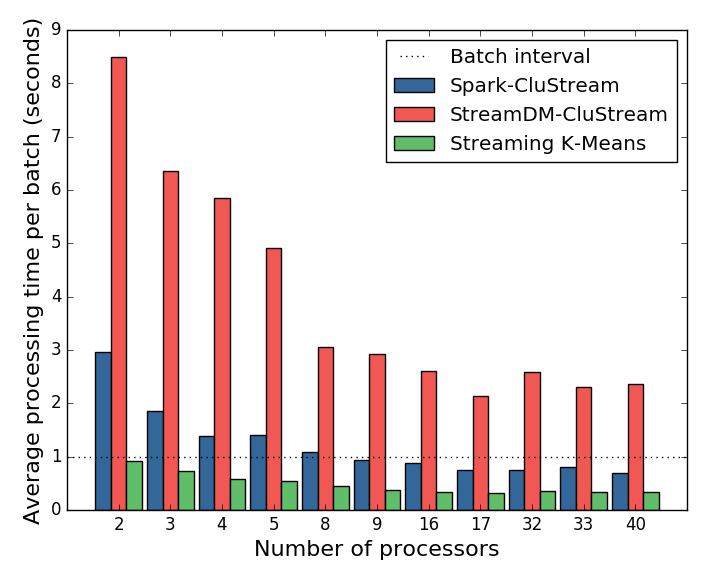
\includegraphics[scale=0.47]{./styles/perfComp100.png}
 \caption{Processing time comparison: $q=20$, $d=100$}
 \label{fig:perfComp100}
\end{figure}

When it comes to higher dimensions, \textit{Spark-CluStream} shows a significant improvement over \textit{StreamDM-CluStream}, which never got to the point were it was stable (below the 1 second mark), as shown in \ref{fig:perfComp100}, it seems to scale as fast as \textit{Spark-CluStream} but it was not enough even with 40 processors. 


\begin{figure}[h!]
 \centering
 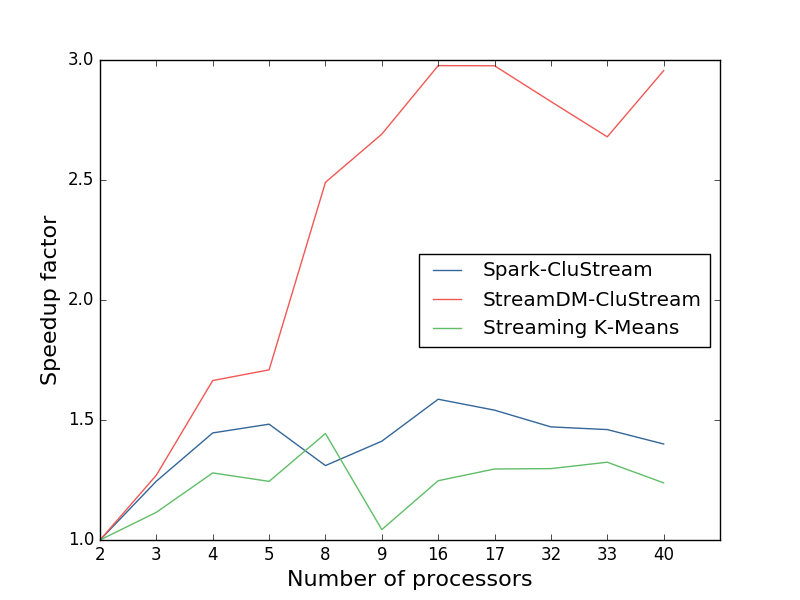
\includegraphics[scale=0.47]{./styles/scalComp2.png}
 \caption{Scalability comparison: $q=20$, $d=2$}
 \label{fig:scalComp2}
\end{figure}

Surprisingly, in Figure \ref{fig:scalComp2}, \textit{StreamDM-CluStream} shows to be able to scale even for this tests, while both \textit{Spark-CluStream} and \textit{Streaming K-Means} seem to struggle taking advantage of using more processors.

\begin{figure}[h!]
 \centering
 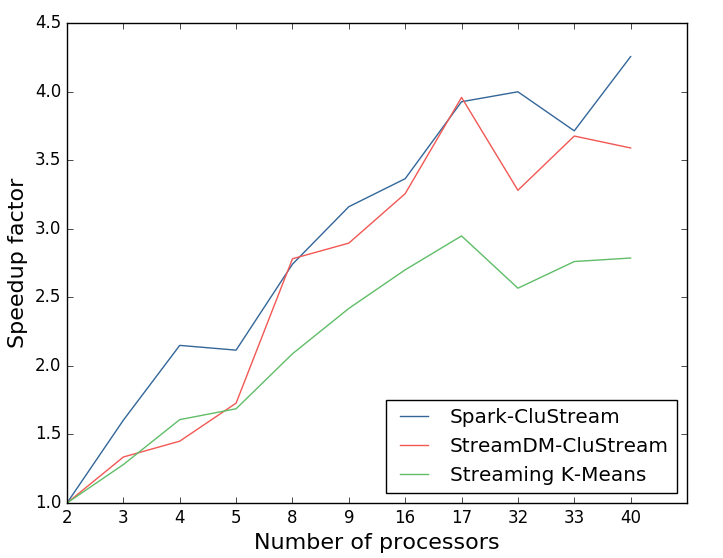
\includegraphics[scale=0.47]{./styles/scalComp100.png}
 \caption{Processing time comparison: $q=20$, $d=100$}
 \label{fig:scalComp100}
\end{figure}

Figure \ref{fig:scalComp100} shows that all three algorithms are able to scale similarly for this test, being \textit{Spark-CluStream} the one having a very slight advantage as it does not slow down as quickly as the other two.



Another interesting comparison, is the processing time per batch of data for a single machine, using a real dataset such as the \textit{Network Intrusion}. Here, communication is less of an issue as all the partitions lie in the same share memory space, and still there are 4 virtual cores in disposition for the algorithms to run. 

The test was performed using a stream speed of 2000 points per batch and with a horizon $H=1$, to match one of the validation tests.

\begin{figure}[h!]
 \centering
 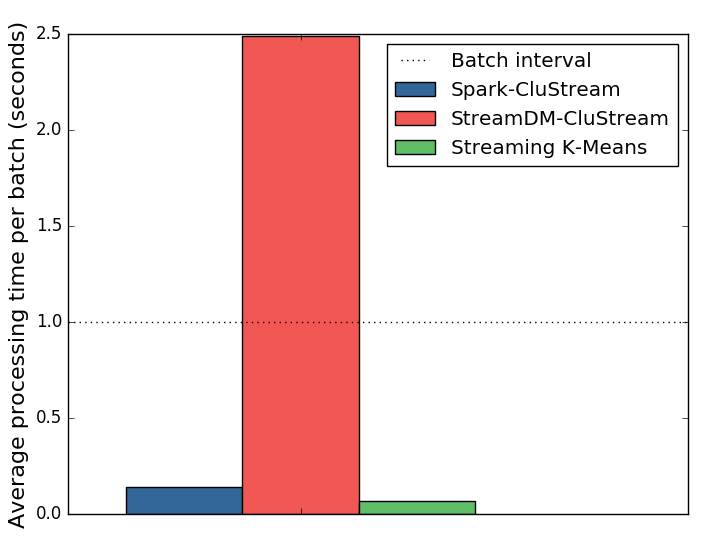
\includegraphics[scale=0.47]{./styles/singlemachine.png}
 \caption{Processing time comparison for a single machine: $q=50$, $d=34$}
 \label{fig:singlemachine}
\end{figure}

The results shown in Figure \ref{fig:singlemachine} are quite remarkable. As \textit{StreamDM-CluStream} shows a very significant disadvantage when using greater numbers of micro-clusters and higher dimensions.

For this single machine test, \textit{Spark-CluStream} was about 18 times faster on average than \textit{StreamDM-CluStream} and about two times slower than \textit{Streaming K-Means} on average.

Another consideration to be made, is that  \textit{Spark-CluStream} saves a snapshot for every batch of data, having to write to disk, while the other two algorithms never access the disk or this matter.



